\documentclass[a4paper, onecolumn, 10pt]{article}

\usepackage[english]{babel}
\usepackage[latin1]{inputenc}
\usepackage[T1]{fontenc}

\usepackage{float} % For controlling figure positions
%\usepackage{etoolbox} % For using conditionals
\usepackage{amsthm, amsmath, amsfonts, amssymb}
\usepackage{fancybox}
\usepackage{color}
\usepackage{cite}
\usepackage{url}

\usepackage{graphicx}
\graphicspath{ {../img/} }

\usepackage[draft, colorinlistoftodos]{todonotes} % Use disable instead of draft to hide todo notes

\usepackage[switch]{lineno}
%\linenumbers

\usepackage{authblk}
\title{Neutral competition boosts chaos in food webs}
\author[1]{Pablo Rodr�guez-S�nchez \thanks{https://pabrod.github.io}} %TODO email or webpage?
\author[1]{Egbert H. van Nes \thanks{egbert.vannes@wur.nl}}
\author[1]{Marten Scheffer \thanks{marten.scheffer@wur.nl}}

\affil[1]{Department of Aquatic Ecology, Wageningen University, The Netherlands}

\begin{document}

\maketitle

\begin{abstract}
\label{sec:Abstract}
Near-neutrality of competition has been proposed to facilitate coexistence of species because it slows down competitive exclusion, thus making it easier for equalizing mechanisms to maintain diverse communities. An unrelated line of work has shown that chaos can promote coexistence of many species in super-saturated communities. By analyzing a set of numerically simulated food webs, here we link those previously unrelated findings. We show that near-neutrality of competition at the prey's trophic level, in the presence of interactions with natural enemies, increases the chances of developing chaotic dynamics. Our results suggest that near-neutrality may promote biodiversity in two ways: through reducing the rates of competitive displacement and through promoting non-equilibrium dynamics.

\paragraph{}
\textit{Keywords}: coexistence, competition, neutral competition, biodiversity paradox.
\end{abstract}

\clearpage

\tableofcontents
%\listoftodos[TODOs]

\clearpage

\section{Background}
\label{sec:Background} 
Ever since Darwin, the idea that species must be sufficiently different to be able to coexist is deeply rooted in the history of biological thinking. Indeed, the principle of competitive exclusion is intuitively straightforward, and elegant mathematical underpinning\cite{MacArthur} helped making it one of the cornerstones of ecological theory. Nevertheless, on a closer examination, natural communities often seem to harbor far more species that may be reasonably explained from niche separation. Plankton communities where many species co-exist with little room for differentiation have served as an early example \cite{Hutchinson, Hutchinson1961} inspiring the legendary ecologist G. Evelyn Hutchinson to ask the simple but fundamental question \textit{"why are there so many kinds of animals?"} \cite{Hutchinson1961}. Since then many mechanisms have been shown to help similar species co-exist. As Hutchinson already proposed himself, fluctuations in conditions may prevent reaching equilibrium at which species would be outcompeted. Also, natural enemies including pests and parasites tend to attack the abundant species more than rare species, and such a "kill the winner"\cite{Winter2010} mechanism promotes diversity by preventing one species to take all the resources and outcompete the rest.

In the extensive literature on mechanisms that can prevent competitive exclusion there are two newcomers that radically different from the rest and have created quite a stir: neutrality and chaos. The neutral theory of biodiversity proposed by Hubbell \cite{Hubbell2001} proposes that species that are entirely equivalent can co-exist in a neutral way because none is able to outcompete the other. The concept of completely equivalent species has met skepticism as it is incompatible with the idea that all species are different. However, it turns out that also "near-neutrality" arises robustly in models of competition and evolution and may boost the chances for co-existence \cite{Scheffer2006, Scheffer2018, Fort2009, Fort2010}. Support for such near-neutrality has been found in a wide range of communities \cite{Scheffer2006, Vergnon2013, Scheffera, Segura2013, Vergnon2012}. The second relatively new and controversial mechanism that may prevent competitive exclusion is "super-saturated co-existence" in communities that display chaotic dynamics \cite{Huisman1999}. This is in a sense analogous to the prevention of competitive exclusion in fluctuating environments, except that deterministic chaos may arise in autonomous non-linear systems without any external perturbation. Although there has been much debate about the question whether such internally driven complex dynamics plays an important role in ecosystems, several studies support the idea that chaos can be an essential ingredient of natural dynamics \cite{Beninca2008}.

Surprisingly, while the potential roles of chaos and neutrality have been intensely debated, no studies seem to have explored how these two fundamental drivers of diversity could be causally related. Here we address this question using simple food-web models. We vary the level of neutrality in the competition between prey species and analyze its effect on the likelihood of generating chaotic dynamics.

\section{Methods}
\label{sec:Methods}

\subsection{Model description}
\label{subsec:Model}

We focused our attention on food webs with two trophic levels, one of consumers and another of prey (see figure \ref{fig:Network}). The consumers predate on the prey, and the prey populations compete among each other for a common source of resources. 

\begin{figure}[h]
	\begin{center}
		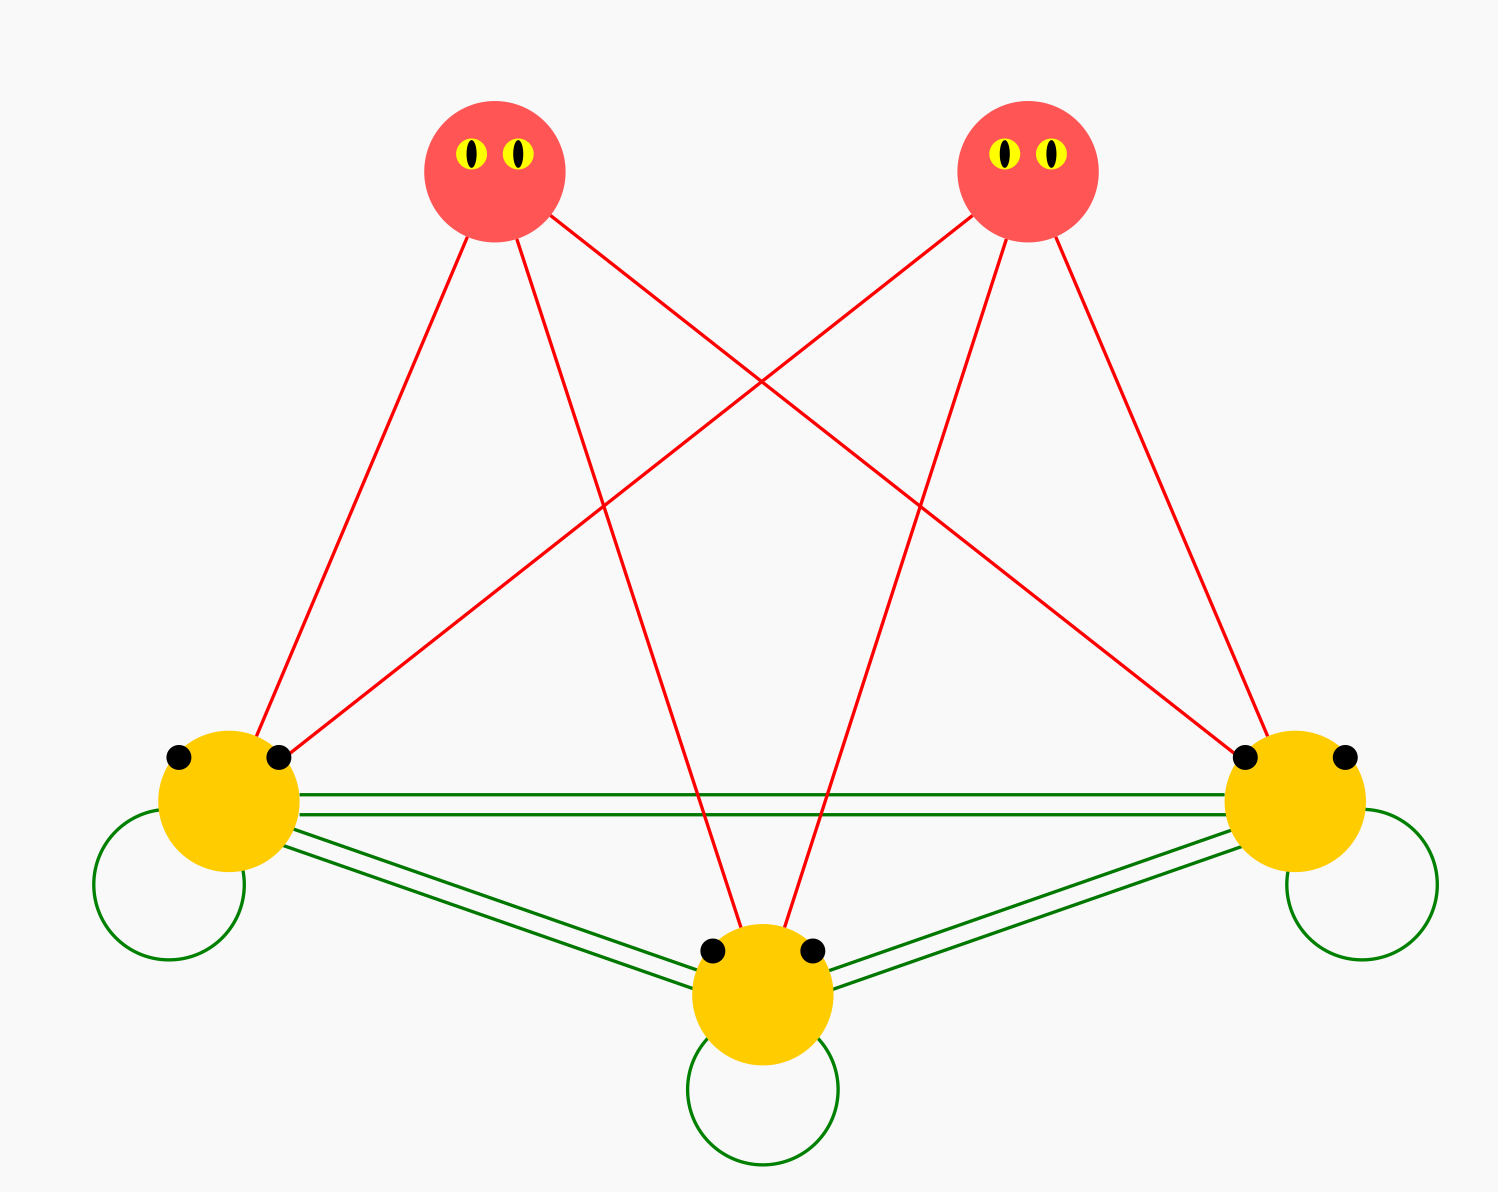
\includegraphics[width=0.7\columnwidth]{net.png}
	\end{center}
	\caption{Example with $2$ consumers and $3$ prey. Each one of the red links represents a predation interaction (coded in the matrix of predator preference coefficients, $ S $). Each green link represents a competition interaction (coded in the matrix of competition coefficients, $ A $). The closed green loops are related with carrying capacity (diagonal elements of $ A $) interpreted here as intra-species competition.}
	\label{fig:Network}
\end{figure}

% Description of the dynamics
The dynamics were modelled as a system of ordinary differential equations. We used the Rosenzweig-MacArthur predator-prey model \cite{Rosenzweig1963} generalized to a higher number of species (see \cite{Scheffer2004} and Online Appendix). 

Our model contains $n_P$ prey species and $n_C$ predator species. The prey's populations grow logistically under the influence of intra and interspecific competition. The intensities of both these competitions are coded in the matrix $A$. The coupling of both groups happens via predation. Obviously, predation has a negative effect for prey and a positive one for predators. The relative preference that predators show to each prey is coded in the matrix $S$. In the absence of prey, the predators' populations just decay exponentially. Prey immigration from neighboring areas has been added to the classical model in order to avoid unrealistic long-stretched cycles with near extinctions \cite{Scheffer2004}.

In mathematical notation, the system reads:

\begin{eqnarray}
\label{eq:SystemUnderStudy}
	\begin{cases} 
	P_i'(t) =  r_i(P) P_i  - P_i \sum_{j = 1}^{n_C} g_j(P) S_{ji} C_j + f & : i = 1..n_P
	\\
	C_j'(t) = - l C_j +  e g_j(P) C_j \sum_{i = 1}^{n_P} S_{ji} P_i & : j = 1..n_C
	\end{cases}
\end{eqnarray}

where $P_i(t)$ represents the biomass of prey species $i$ at time $t$ and $C_j(t)$ the biomass of predator species $j$ at time $t$. The auxiliary functions $r_i(P)$ and $g_j(P)$ have been respectively chosen to generalize the logistic growth and the Holling type II saturation functional response \cite{Edelstein-Keshet} to a multispecies system when inserted into equation \ref{eq:SystemUnderStudy}. They are defined as:

\begin{eqnarray}
\label{eq:HollingGenerator}
	r_i(P) = r \left( 1 - \frac{1}{K} \sum_{k=1}^{n_P} A_{ik} P_k \right)
	\\
	g_j(P) = \frac{g}{\sum_{i=1}^{n_P} S_{ji} P_i + H}
\end{eqnarray}

For details about the parameters used, please refer to subsection \ref{subsec:Parameterization}. For a detailed derivation of equation \ref{eq:SystemUnderStudy}, see Online Appendix.

\begin{figure}
	\begin{center}
		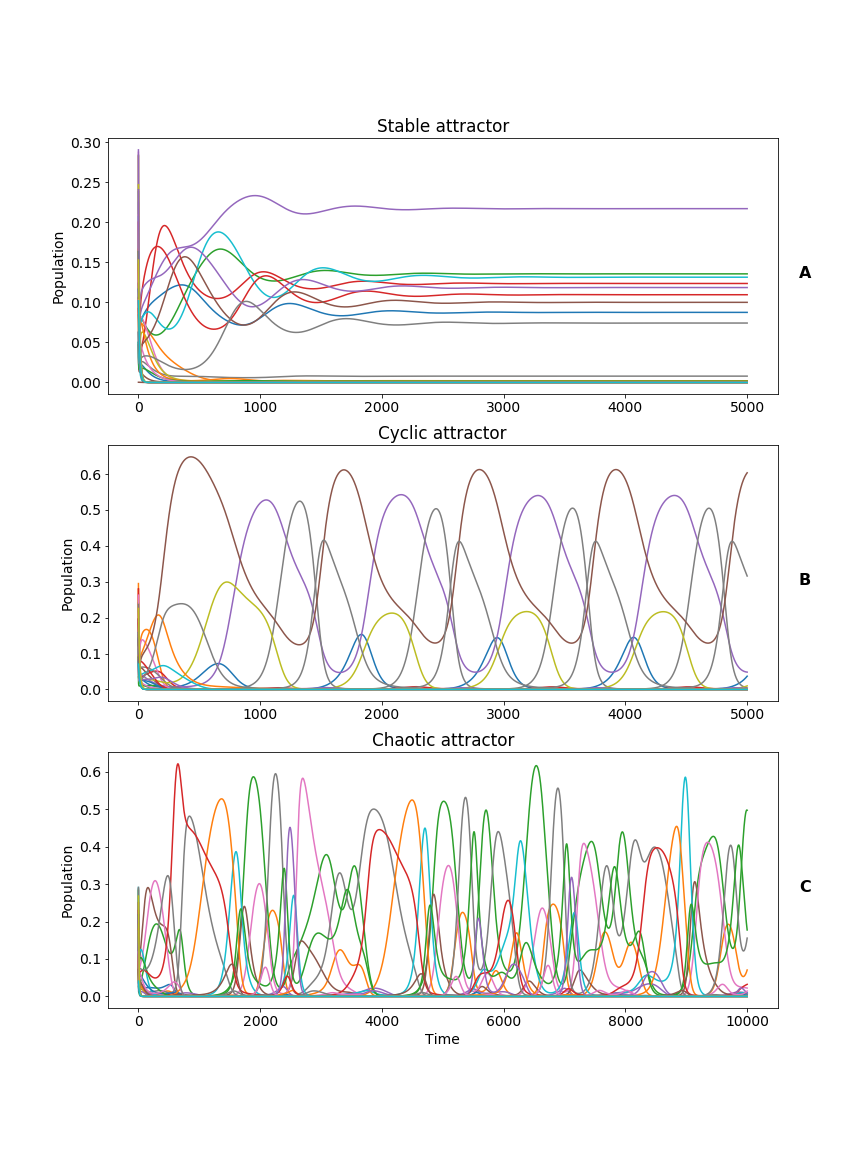
\includegraphics[width=1\columnwidth]{ts.png}
	\end{center}
	\caption{Our model generates time series of the population of each species. The time series can be classified in $3$ qualitative types depending on their asymptotic behavior: \textit{stable}, \textit{periodic} and \textit{chaotic}. In \textbf{panel A}, the system reaches a stable attractor after a transient time. In \textbf{panel B}, a periodic attractor, with an approximate period of 1000 days, is reached after the transient time. The system in \textbf{panel C} never reaches a stable nor a cyclic attractor, but a chaotic one.}
	\label{fig:TimeSeries}
\end{figure}

\subsection{Parameterization}
\label{subsec:Parameterization}
We parameterized our model as a freshwater plankton system based on Dakos' model \cite{Dakos2009b}. Dakos' model uses a Rosenzweig-McArthur multi-species model with two trophic levels, and parameterizes it to describe a zooplankton-phytoplankton system. Unlike Dakos, who uses seasonally changing parameters, our parameters were assumed to be constant for simplicity (see table \ref{tab:Parameters}).

\begin{table}[H]
	\begin{center}
		\resizebox{\columnwidth}{!}{
		\begin{tabular}{|c|c|c|c|}
			\hline
			\textbf{Symbol} & \textbf{Interpretation} & \textbf{Value} & \textbf{Units} \\
			\hline
			$r$ & Maximum growth rate & $0.50$ & $d^{-1}$ \\
		    \hline
			$K$ & Carrying capacity & $10.00$ & $ mg \ l^{-1} $ \\
			\hline
			$g$ & Predation rate & $0.40$ & $d^{-1}$\\
			\hline
			$f$ & Immigration rate & $10^{-5}$ & $mg \ l^{-1} \ d^{-1}$\\
			\hline
			$e$ & Assimilation efficiency & $0.60$ & $1$\\
			\hline
			$H$ & Half-saturation constant & $2.00$ & $ mg \ l^{-1} $\\
		    \hline
			$l$ & Predator's loss rate & $0.15$ & $d^{-1}$\\
			\hline
		    $S$ & $ n_C \times n_P $ predator preference matrix & $S_{ij} \in (0,1)$ & $1$\\
		    \hline
   		    $A$ & $ n_P \times n_P $ competition matrix & See section \ref{subsubsec:CompetitionParameter} & $1$\\
		    \hline
		\end{tabular}}
	\end{center}
	\caption{Values and meanings of the parameters used in our numerical experiment}
	\label{tab:Parameters}
\end{table}

\subsubsection{Competition matrix}
\label{subsubsec:CompetitionParameter}

Our main purpose is to analyze the effect of different degrees of heterogeneity in the matrix competition on the long term dynamics exhibited. In order to simulate and quantify this heterogeneity, we introduce the competition parameter $ \epsilon $. This dimensionless parameter was used to build a competition matrix $A$ whose diagonal terms are identically $ 1 $, and whose non-diagonal terms are drawn from a uniform probability distribution centered at $ 1 + \epsilon $ and with a given width (here we chose $ w = 0.2$). In mathematical terms: the elements of our competition matrix $A$ were drawn from probability distributions whose shape depend on the value of $\epsilon$.

%TODO Maybe send figure to appendix
Defined this way, the parameter $\epsilon$ allows us to travel continuously from strong dominant intraspecific ($ \epsilon < 0$) to strong interspecific competition ($ \epsilon > 0$), meeting neutral competition near $\epsilon = 0$ (see figure \ref{fig:CompetitionParameter}).

\begin{figure}[H]
	\begin{center}
		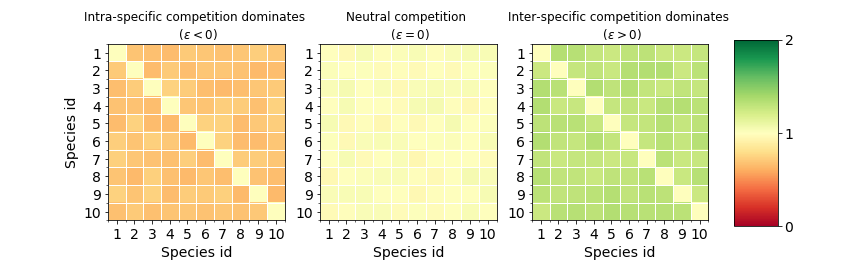
\includegraphics[width=1\columnwidth]{epsilon_all.png}
	\end{center}
	\caption{The competition matrix on the left is a clear case of dominant intraspecific competition. The central one represents a case of neutral competition. The matrix in the right panel shows a case of dominant interspecific competition. The difference between them is the relative size of the non-diagonal elements respective of the diagonal ones. This qualitative property of the competition matrices is controlled by the parameter $\epsilon$.}	
	\label{fig:CompetitionParameter}
\end{figure}

\subsection{Numerical experiment}
\label{subsec:NumericalExperiment}

Depending on the parameters and the initial conditions, the system described in equation \ref{eq:SystemUnderStudy} can give rise to three types of asymptotic behavior, each of them roughly corresponding to a different type of attractor (see figure \ref{fig:TimeSeries}). The first one, a stable point attractor, generates a constant species composition. Secondly, limit cycle (and limit tori) attractors give rise to periodically (or quasiperiodically) changing species composition. Lastly, we'll refer as chaotic to attractors not fitting in any of the previous categories.

Our target is to estimate the probability of reaching one of such chaotic attractors under different assumptions about intraspecific competition. In order to achieve this, we simulated several ecosystems with different initial conditions and predation coefficients $S_{ji}$, drawn using the same competition parameter $\epsilon$ (defined in section \ref{subsubsec:CompetitionParameter}).

Numerical methods are used to integrate the equation \ref{eq:SystemUnderStudy}. Starting with random initial conditions (redrawn after every run), a first stabilizing run of $ 2000 $ days is generated in order to get closer to the attractor. Simulating for $ 5000 $ more days, we obtain time series as the ones in figure \ref{fig:TimeSeries}. 

%TODO point to appendix
In the exploratory phase of this research three parallel approaches to chaos detection were followed: Lyapunov exponents estimation \cite{Strogatz1994}, Gottwald-Melbourne \textit{0-1} test \cite{Gottwald2009} and visual inspection (see Online Appendix). Despite differences in the exact probabilities, the three of them led us to the same qualitative conclusions. We found the results of the Gottwald-Melbourne test most consistent with visual inspection. We called chaotic all those time series complicated enough to trigger the Gottwald-Melbourne test. Using this approach, we classified each individual simulation as \textit{chaotic} or \textit{non-chaotic}. Our numerical experiment was repeated $ 200 $ times per competition parameter, and thus, generating $ 200 $ different competition matrices per competition parameter value. The ratio of attractors found to be chaotic can be used to estimate the probability of ecosystems of a given degree of heterogeneity developing chaotic asymptotic behavior.

Additionally, the experiment was repeated for food webs of different sizes. In our simulations, we kept a ratio of 2:3 for the number of species at the consumer and the prey level.

For the sake of reproducibility, we provide a \textit{GitHub} link to the analysis scripts used\footnote{https://github.com/PabRod/Chaos-and-neutrality}.

\section{Results}
\label{sec:Results}
Plotting the probability of chaos against the competition parameter (see figure \ref{fig:Results}), we observe a clear maximum around $ \epsilon = 0 $. The likelihood of chaotic behaviour for neutral competition at the prey's trophic level is thus higher than for dominant inter or intraspecific competition. This result remains true for systems with a different number of species (figures \ref{fig:Results} and \ref{fig:Contour}).

The overall likelihood of chaos, which can be interpreted as the area under the curve in figure \ref{fig:Results}, increases with the size of the food web. This effect should not be surprising: the more dimensions the phase space has, the easier is to fulfill the requirements of the complex geometry of a chaotic attractor \cite{Strogatz1994}. We can understand this intuitively as increasing the available room for the trajectories to pack closer and closer without ever crossing each other nor collapsing to a point. Even in those higher dimensional cases, there is still a clear maximum at neutral competition.

% Weak and strong interspecific competition
Another local maximum was observed around $ \epsilon = -1 $. This means that weak competitive coupling, in our model, also promotes chaos.

Between both local maxima there is obviously a local minimum whose exact position differed between experiments.

\begin{figure}
	\begin{center}
		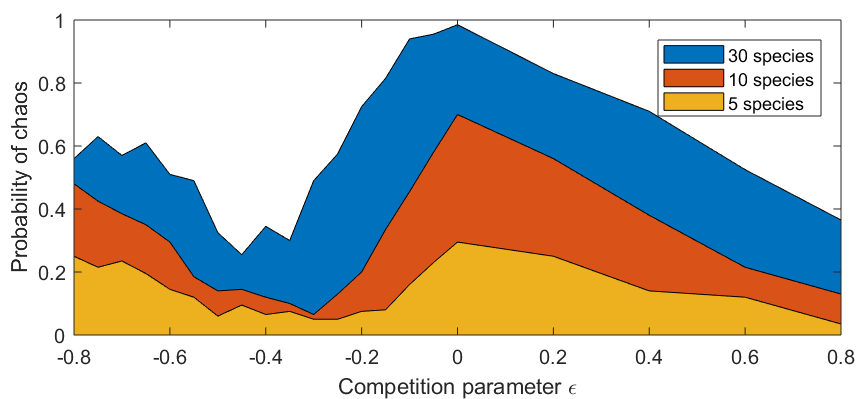
\includegraphics[width=1\columnwidth]{results.png}
	\end{center}
	\caption{Results for a low, medium and high dimensional system. Notice how the probability of chaos has a local maximum around $\epsilon = 0$. The overall probability of chaos, understood as the area under the curve, grows with the system size. The local maximum stays at $\epsilon = 0$ even for systems with a high number of species.}
	\label{fig:Results}
\end{figure}

\begin{figure}
	\begin{center}
		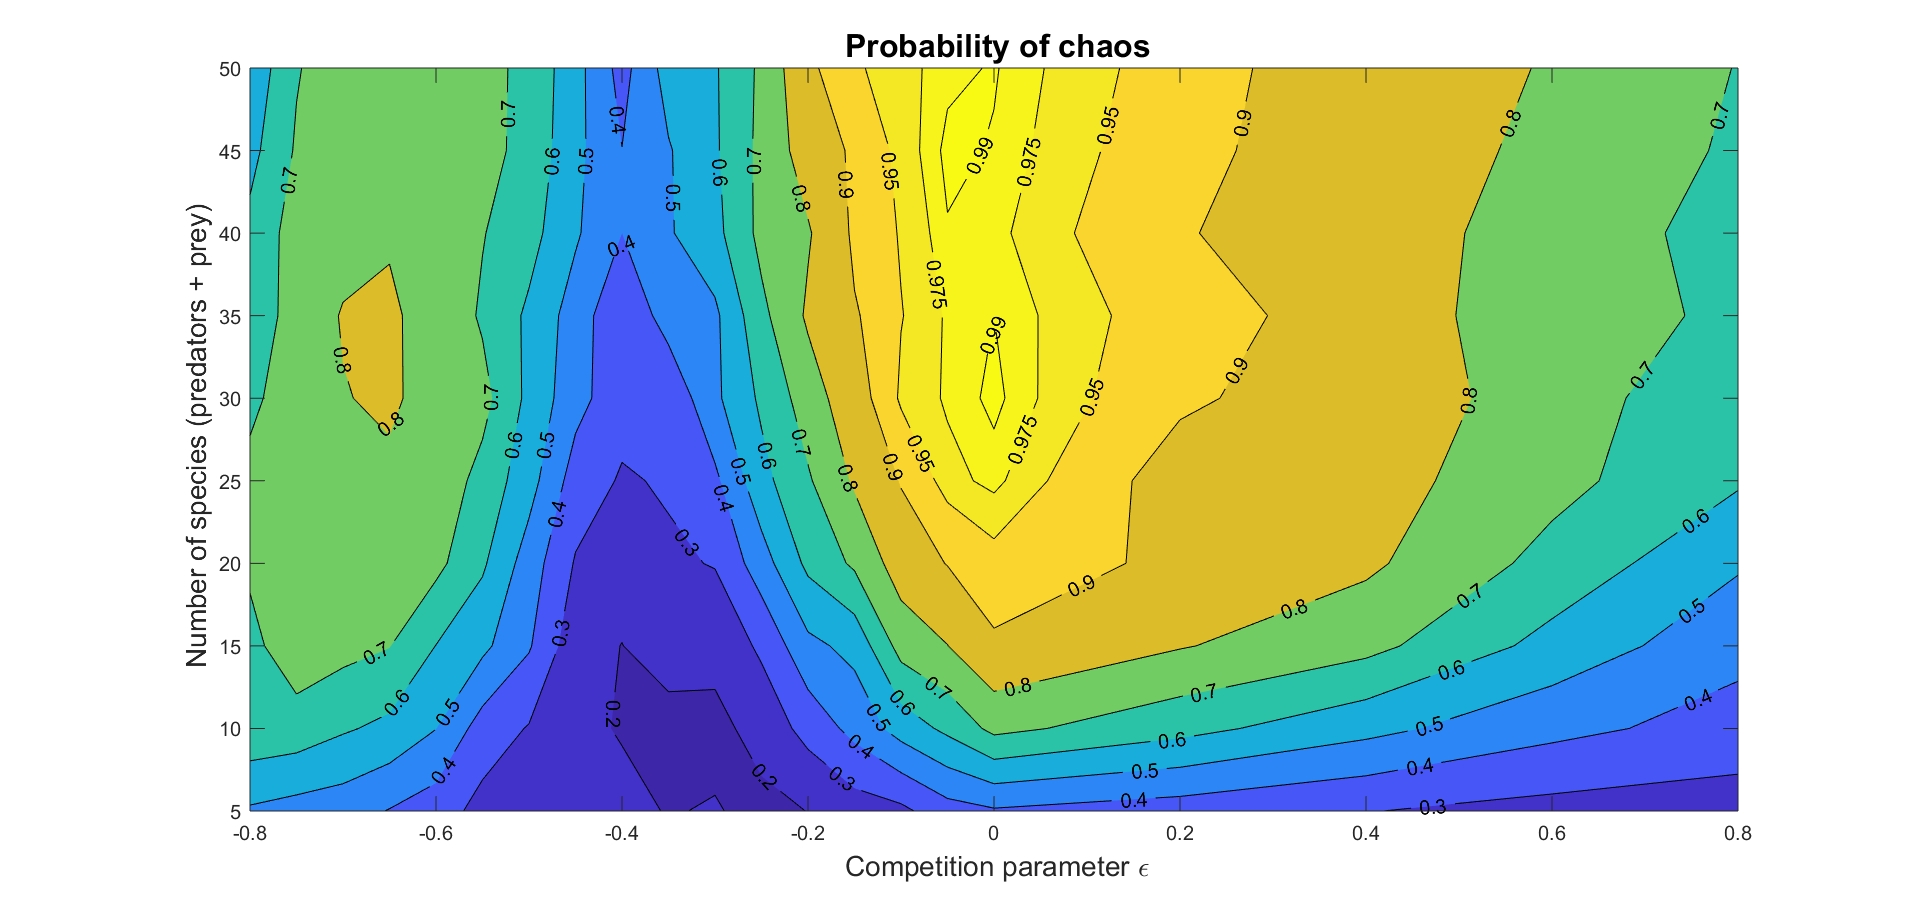
\includegraphics[width=1\columnwidth]{contour.png}
	\end{center}
	\caption{Contour map showing the probability of chaos for various competition parameters (horizontal axis) and number of species (vertical axis). The consumers' population is fixed as $ 2/3 $ of the prey's population. Notice that chaotic attractors appear more easily (i.e., for smaller systems) the closer is the competition to neutral (i.e., $ \epsilon = 0 $).}
	\label{fig:Contour}
\end{figure}

\section{Discussion}
\label{sec:Discussion}
% Our claims
The asymptotic dynamics of our model are affected by the strength of intraspecific competition compared to interspecific competition is. Interestingly, we find that competition closer to neutrality leads to chaotic behaviour. This suggests that in a system with predation, near-neutrality at the competition level may increase the probability of complex dynamics if the species are not equally prone to predation. Provided that the competitive exclusion principle rests on the assumption of equilibrium, near-neutrality reduces the chances of the principle to be applicable, improving the chance for a higher number of coexisting species if dynamics are chaotic \cite{Huisman1999}. Additionaly, this observation suggests that the hypothesis of non-equilibrium and Hubbell's hypothesis of neutrality are not completely independent. Our model shows another local maximum for the probability of chaos for weak competition coupling. We consider this a reasonable result, as predation is known to be the main driver of chaos in this kind of models \cite{Scheffer2004}.

%% Limitations
% Why two levels?
In the spirit of mathematical modelling, we chose the simplest realization required for the effects to be observed. We didn't use Allee effect, nor noise, and the functional form of each term has been chosen to account for satiation and saturation in the simplest possible ways. The choice of a two-level model may seem in contradiction with the pursue of simplicity, but actually it is a fundamental requirement for the effect under research to take place. In the absence of a predator level, chaos will never develop in a model with neutral competition. The reason for this is that if all interactions become equally strong, the differences among species at the same trophic level fade out. This makes labeling each species meaningless, and thus the prey-only system can be reduced just to one differential equation, that of the total prey population (see Online Appendix for details). Using the Poincar�-Bendixson theorem, it can be proven that autonomous systems with less than $3$ dimensions cannot exhibit chaos \cite{Strogatz1994}.

% Choice of interaction parameters: modularity
For simplicity, both the competition and predation parameters were drawn from probability distributions. The interactions in our system can be interpreted as a weighted network with a high connectivity. In nature, trophic networks tend to show modular structure with various clusters \cite{Thebault2010}. Our simplified model could be interpreted as representing one of the densely connected modules.

% Choice of interaction parameters: randomness
It is known that the asymptotic behaviour of this kind of systems can be very sensitive to the parameters choice. In particular, introducing correlations between parameters can greatly modify the probabilities of chaotic attractors to be reached (see for instance \cite{Huisman2001}, in response to the letter \cite{Schippers2001}). In the present paper we didn't introduce any correlation, i.e., all our random parameters were drawn independently from the others. Studying the effect of different physiological scenarios (in the sense of \cite{Huisman2001}, that is, constrains between the parameters) on the probabilities of chaos could be a continuation to this paper.

% Role of symmetry
%TODO Effects of symmetry, show or not mention
%It may be worth noting that the position of both the maxima we've found (i.e.: $ \epsilon = -1 $ and $ \epsilon = 0 $) have something in common: the community matrix $ A $ at those values of the parameter is very symmetric in both cases. It will be interesting to develop a similar method that, instead of varying neutrality, varies the less restrictive property of symmetry.
%\todo[inline, color=blue!25, caption={Effects of symmetry}]{\textbf{Egbert}: Good chance that a reviewer says: nice these suggestions, but why do they not show it here? \\ \textbf{Pablo}: Remove or do? \\ \textbf{Egbert}: up to you. Maybe it is not so difficult to perform the same analysis imposing symmetry}

% Chaos detection
Due to the large number of simulations made, we had to rely on automatic methods for detecting chaos. Automatic detection of chaos by numerical methods has fundamental limitations, especially for high dimensional systems like ours. Most of them can be boiled down to the fact that, in general, numerical methods cannot distinguish robustly between long, complicated transients and genuine chaos. We think that our approach to chaos detection, despite being open to improvement, suffices to detect the overall patterns.

% Concluding remark
The paradox of biodiversity is a tremendously complex scientific problem. With these model exercises we definitely do not claim to have solved it, but we show that predation in combination with neutral competition may increase the probability of chaos, and thereby increase the number of coexisting species.

\textbf{Marten's suggestion:} Our results suggest a fundamentally new way in which near-neutrality may promote biodiversity. In addition to weakening the forces of competitive exclusion \cite{Scheffer2018}, our analyses reveal that near neutrality may boost the chances for chaotic dynamics. As chaos in turn may facilitate super-saturated co-existence, our findings point to a potentially widespread mechanism of maintaining biodiversity.

\begin{figure}
	\begin{center}
		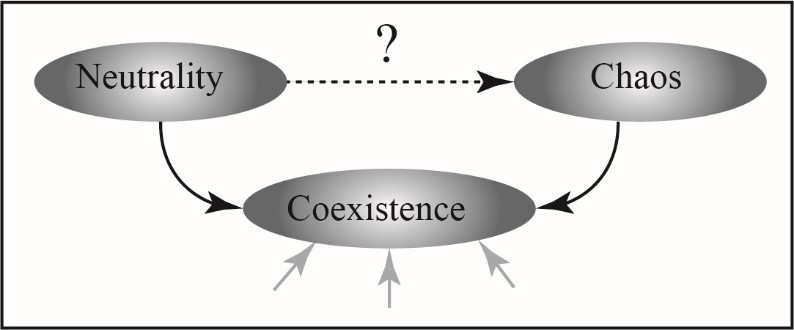
\includegraphics[width=0.5\columnwidth]{gap.jpg}
	\end{center}
	\caption{Suggested figure}
	\label{fig:GapInKnowledge}
\end{figure}

% Is chaos more resilient?
%Additionally, we are implicitly assuming without a proof that chaotic ecosystems can have more species %than non-chaotic ones\todo{Stronger concluding remark required}.
%\todo[inline, caption={This is well known in math}]{There are mathematical reasons for this to be true. Keywords: uniformly hyperbolic dynamical systems, Anosov maps, Arnold's cat map.}
%%TODO there are mathematical reasons for this to be true. Keywords: uniformly hyperbolic dynamical systems, Anosov maps, Arnond's cat map

%%TODO A possible continuation of this research may be the setting of two indepedent ecosystems, one of them chaotic and the other one non-chaotic, and allow them to interact at some point of time (simulating an invasion), in order to assess how much of each of the original ecosystems survives to this traumatic event. This is a good idea, but I think testing for resilience is too far from this study to put it here. You could instead refer to the discussions about  Huismans paper (Schippers, P., A. M. Verschoor, M. Vos, and W. M. Mooij. 2001. Does "supersaturated coexistence" resolve the "paradox of the plankton"? Ecology letters 4:404-407. and Huismans reply) {Schippers2001}

\section{Acknowledgements}
\label{sec:Acknowledgements}
The preliminary analysis of this model were performed using GRIND for Matlab (http://www.sparcs-center.org/grind). Additionally, we thank Tobias Oertel-J�ger, Sebastian Wieczorek, Jeroen Lamb, Martin Rasmussen, Cristina Sargent, Jelle Lever, Moussa N'Dour and Sebastian Bathiany for their useful comments and suggestions. 

This work was supported by funding from the European Union's \textit{Horizon 2020} research and innovation programme for the \textit{ITN CRITICS} under Grant Agreement Number 643073.

\clearpage

\section{Online appendix}
\label{sec:Appendix}

\subsection{Generalized multispecies predation models}
\label{subsec:GeneralizedModels}

\subsubsection{General properties of predation models}
\label{subsubsec:GeneralPropertiesOfPredation}

Most predation models based on differential equations follow a structure like this:

\begin{eqnarray}
\label{eq:CommonStructure}
	\begin{cases}
	P'(t) = Growth(P) - Predation(P,C)
	\\ 
	C'(t) = -Loss(C) + GrossGrowth(P,C)
	\end{cases}
\end{eqnarray}

where $P$ represents the biomass of the prey population, and $C$ the biomass of the consumer/predator population. The functional dependences have been explicitly written in order to remark the fact that the coupling of the system happens via the $Predation$ and $GrossGrowth$ terms.

It is important to note that, in models like this, all deaths at the prey's level are due to predation. All deaths caused by predation are invested in consumer's growth. Therefore the following relation must be true:

\begin{equation}
\label{eq:InnerEnergyFlow}
	GrossGrowth(P,C) = e \cdot Predation(P,C)
\end{equation}

where $e$ represents the efficiency of the energy transfer process. Equation \ref{eq:InnerEnergyFlow}, when plugged into \ref{eq:CommonStructure}, yields:

\begin{equation}
\label{eq:AllEnergyFlow}
	e P'(t) + C'(t) = e \cdot Growth(P) - Loss(C)
\end{equation}

Equation \ref{eq:AllEnergyFlow} allows us to think of our system as an open system from the point of view of thermodynamics. Here $Growth$ is the only source of the system, and $Loss$ is the only sink (see figure \ref{fig:EnergyFlow}). All the energy exchange due to predation stays inside the system, so predation can be considered a closed subsystem.

\begin{figure}
	\begin{center}
		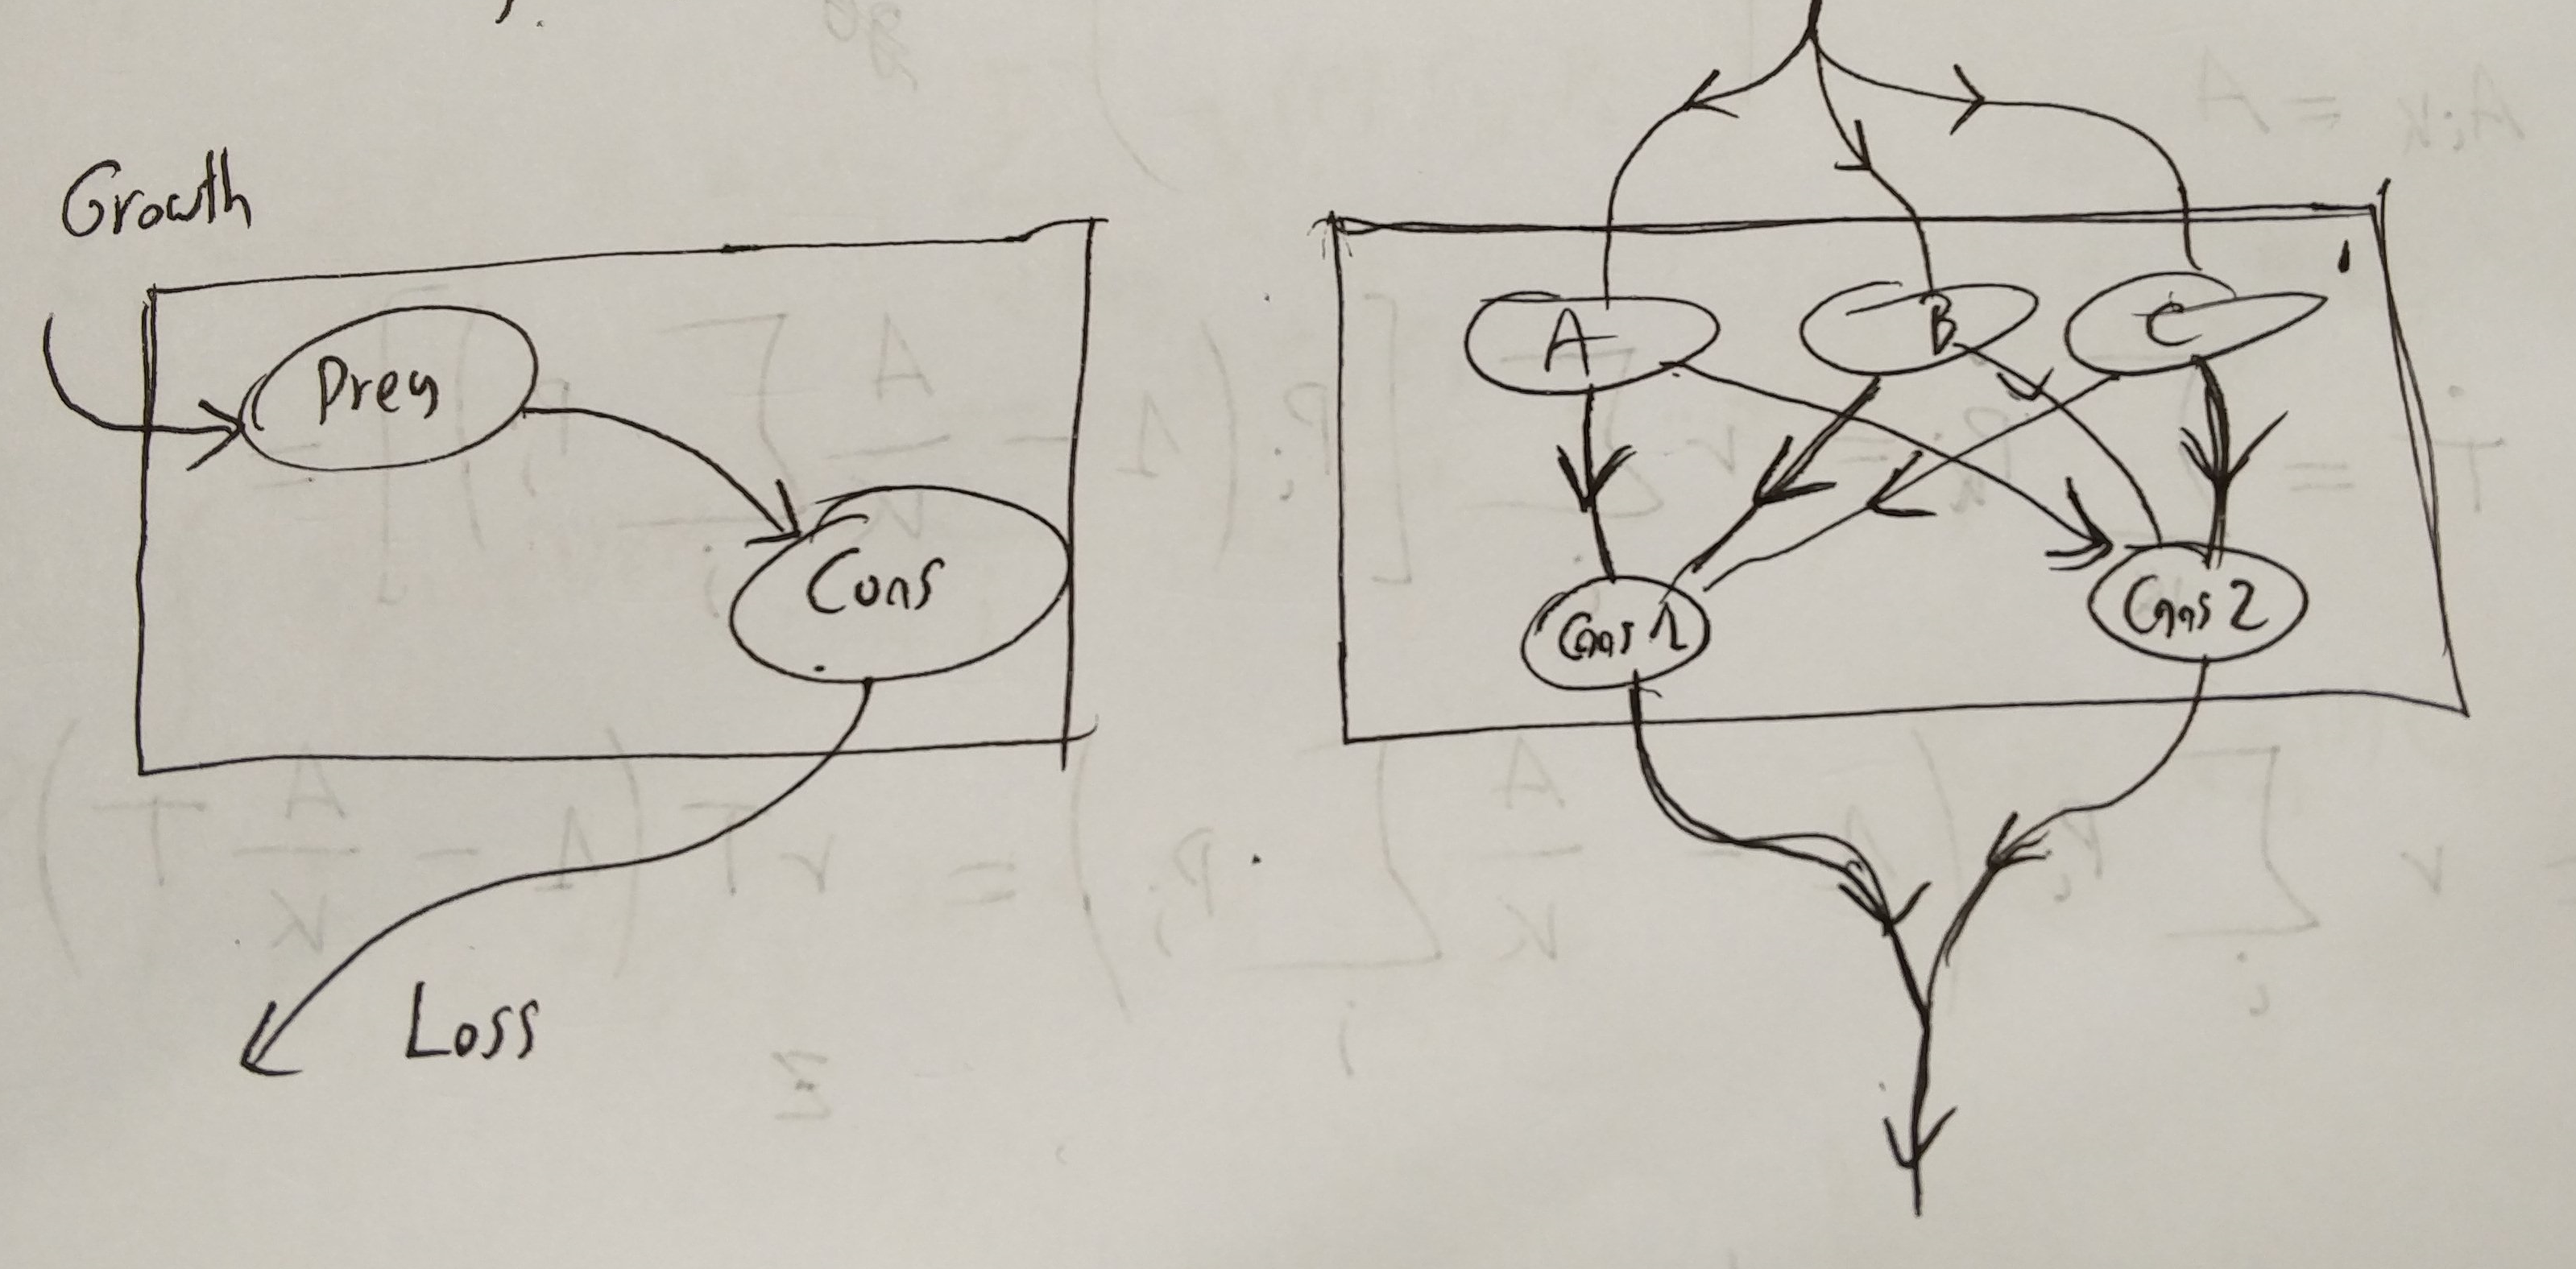
\includegraphics[width=1\columnwidth]{energyflow.png}
	\end{center}
	\caption{Plot showing the energy flow for a two species and a multispecies system.}
	\label{fig:EnergyFlow}
\end{figure}

We can generalize this basic structure to multispecies, two trophic levels systems. First, we'll go back to equation \ref{eq:CommonStructure} and just add more rows, while we are specially careful with the variables in the functional relations:

\begin{eqnarray}
\label{eq:CommonStructureMulti}
	\begin{cases}
	P_i'(t) = Growth_i(P) - Predation_i(P,C) & : i = 1..n_P
	\\ 
	C_j'(t) = -Loss_j(C_j) + GrossGrowth_j(P,C_j) & : j = 1..n_C
	\end{cases}
\end{eqnarray}

where now $i$ runs from $1$ to the number of prey $n_P$ and $j$ from $1$ to the number of consumers $n_C$. Here, we've used $P_i$ to denote the population of the prey labeled by $i$, and $P$ for the vector containing all prey populations. Notice that, while the $Growth$ term can involve competition (and thus, depends on the whole vector $P$), the $Loss$ term for species $j$ depends only in the population of that species (i.e.: $C_j$), regardless of the rest.

Requiring once again our predation to be fully invested in consumer's growth, we find the following generalization of equation \ref{eq:InnerEnergyFlow}:

\begin{equation}
\label{eq:InnerEnergyFlowMulti}
	\sum_{j = 1}^{n_C} GrossGrowth_j(P,C_j) = \sum_{i = 1}^{n_P} e_i \cdot Predation_i(P,C)
\end{equation}

Using \ref{eq:InnerEnergyFlowMulti} and \ref{eq:CommonStructureMulti}, it is easy to prove that the multispecies generalization of \ref{eq:AllEnergyFlow} is:

\begin{equation}
\label{eq:AllEnergyFlowMulti}
	\sum_{i = 1}^{n_P} e_i P_i'(t) + \sum_{j = 1}^{n_C} C_j'(t) = \sum_{i = 1}^{n_P} e_i \cdot Growth_i(P) - \sum_{j = 1}^{n_C} Loss_j(C_j)
\end{equation}

The intuitive interpretation is, again, that the sinks and sources of energy in our systems are the total $Loss$ and $Growth$.

Restriction \ref{eq:InnerEnergyFlowMulti} (or equivalently, \ref{eq:AllEnergyFlowMulti}) can be used to generalize realistic functional forms for the coupling terms. As the coupled terms that are related to predation, those terms are the very core of this models.

\subsubsection{Lotka-Volterra equations}
\label{subsubsec:LotkaVolterra}

The most basic model of predation is the Lotka-Volterra system of equations:

\begin{eqnarray}
\label{eq:LotkaVolterra}
	\begin{cases}
	P'(t) = r P - g P C
	\\ 
	C'(t) = - l C + e g C P
	\end{cases}
\end{eqnarray}

Where $r$ represents the growth rate of the prey, $g$ the grazing rate of the predator against the prey, $l$ the loss rate of the predator and $e$ the efficiency conversion factor.

It is trivial to prove that the Lotka-Volterra model satisfies the requirements shown in subsection \ref{subsubsec:GeneralPropertiesOfPredation}. 

\subsubsection{Multispecies Lotka-Volterra equations}
\label{subsubsec:LotkaVolterraMulti}

Lotka-Volterra equations can be generalized to a model with multiple species by noting that each prey will be affected by all consumers, and each consumer will be affected by all prey. In order to code the strength of this interactions, we introduce the matrix $S$, whose element $S_{ji}$ gives the strength of the coupling of consumer $j$ and prey $i$. As a consequence: for prey dynamics, this matrix is scanned row-wise, while for predators it is scanned column-wise. The generalized system looks like:

\begin{eqnarray}
\label{eq:LotkaVolterraMulti}
	\begin{cases}
	P_i'(t) = r_i P_i - P_i \sum_{j = 1}^{n_C} g_j S_{ji} C_j & : i = 1..n_P
	\\ 
	C_j'(t) = - l_j C_j +  g_j e_j C_j \sum_{i = 1}^{n_P} S_{ji} P_i  & : j = 1..n_C
	\end{cases}
\end{eqnarray}

The fulfillment of condition \ref{eq:InnerEnergyFlowMulti} is again easily proven.

In this model, all terms can grow without boundaries. This is not only unrealistic, but also creates some problems from the sole point of view of mathematical stability.

\subsubsection{Rosenzweig-MacArthur model}
\label{subsubsec:Rosenzweig-MacArthur}
The Rosenzweig-MacArthur predator-prey model improves the previous model by adding boundaries to the terms' dependency on the prey population. This is achieved by encapsulating $P$ inside saturating functions. In particular, the growth rate $r$ now depends on $P$, and the grazing rate $g$ in the coupling terms is now a function of $P$ (see equation \ref{eq:RosMac2levels} and compare it with \ref{eq:LotkaVolterra}).

\begin{eqnarray}
\label{eq:RosMac2levels}
	\begin{cases}
	P'(t) = r(P) P - g(P) P C
	\\ 
	C'(t) = - l C + e g(P) C P
	\end{cases}
\end{eqnarray}

Once again, condition \ref{eq:InnerEnergyFlow} is trivially fulfilled independently of the functional form of $r(P)$ and $g(P)$. If those both functions are chosen appropriately, we avoid unbounded growths. Typically a logistic growth form is chosen for $r(P)$, that is, $r(P) = r_0 \left(1 - \frac{P}{K} \right)$, and a Holling type II functional form for the grazing $g(P)$, that is, $g(P) = \frac{g_0}{P+H}$ (see, for instance, \cite{Edelstein-Keshet}). After making this choices, our system takes its classical form:

\begin{eqnarray}
\label{eq:RosMac2classic}
	\begin{cases}
	P'(t) =  r P \left( 1 - \frac{P}{K} \right) - g C \frac{P}{P + H}
	\\ 
	C'(t) = - l C + e g C \frac{P}{P + H}
	\end{cases}
\end{eqnarray}

\subsubsection{Multispecies Rosenzweig-MacArthur model}
\label{subsubsec:Rosenzweig-MacArthurMulti}

Noticing the similarities between equations \ref{eq:LotkaVolterra} and \ref{eq:RosMac2levels}, the latter can be generalized in the same fashion as we did to obtain \ref{eq:LotkaVolterraMulti}, yielding:

\begin{eqnarray}
\label{eq:RosMacMulti}
	\begin{cases}
	P_i'(t) = r_i(P) P_i - P_i \sum_{j = 1}^{n_C} g_j(P) S_{ji} C_j & : i = 1..n_P
	\\ 
	C_j'(t) = - l_j C_j +  g_j(P) e_j C_j \sum_{i = 1}^{n_P} S_{ji} P_i  & : j = 1..n_C
	\end{cases}
\end{eqnarray}

Written like this, it is easy to see that the condition \ref{eq:InnerEnergyFlowMulti} is fulfilled. 

Regarding the proper functional forms of $r_i(P)$ and $g_j(P)$, our growth term has to take into account both the inter and intraspecific competition. This can be easily modelled by choosing:

\begin{equation}
\label{eq:r}
	r_i(P) = r_i \left( 1 - \sum_{k=1}^{n_P} A_{ik} P_k \right)
\end{equation}

where the matrix elements $A_{ik}$ account for the intensity of the competition caused by species $k$ on species $i$. Thus, non-diagonal elements account for interspecific competition, and diagonal ones for intraspecific competition.

We hypothesize that the grazing rates corresponding to predator $j$, that is, $g_j(P)$, follow a Holling type II functional response dependent on the total consumption of prey by predator $j$:

\begin{eqnarray}
\label{eq:g}
	g_j(P) = \frac{g_j}{\sum_{i=1}^{n_P} S_{ji} P_i + H_j}
\end{eqnarray}

\subsubsection{Summary}
\label{subsubsec:SummaryPredation}

\begin{table}[H]
\label{tab:SummaryPredation}
	\begin{center}
		\resizebox{\columnwidth}{!}{
			\begin{tabular}{|c|c|c|} \hline 
				 & Two species & Multispecies \\ 
				\hline 
				Lotka-Volterra & $\begin{cases}P'(t) = r P - g P C\\ C'(t) = - l C + e g C P\end{cases}$ & $\begin{cases} P_i'(t) = r_i P_i - P_i \sum_{j = 1}^{n_C} g_j S_{ji} C_j \\ C_j'(t) = - l_j C_j +  g_j e_j C_j \sum_{i = 1}^{n_P} S_{ji} P_i \end{cases}$ \\ 
				\hline 
				Rosenzweig-MacArthur & $\begin{cases}P'(t) = r(P) P - g(P) P C\\C'(t) = - l C + e g(P) C P\end{cases}$ & $\begin{cases} P_i'(t) = r_i(P) P_i - P_i \sum_{j = 1}^{n_C} g_j(P) S_{ji} C_j \\ C_j'(t) = - l_j C_j +  g_j(P) e_j C_j \sum_{i = 1}^{n_P} S_{ji} P_i \end{cases}$  \\
			\hline  \end{tabular}}
	\end{center}
	\caption{Summary table with the different types of predation models studied. Written this way, the parallelisms are obvious. In multispecies models, the index $i$ runs from $1$ to $n_P$, and $j$ from $1$ to $n_C$. The functional forms of $r_i(P)$ and $g_j(P)$ are given in equations \ref{eq:r} and \ref{eq:g}}
\end{table}

\subsection{Melbourne-Gottwald 0-1 test in a nutshell}
\label{subsec:z1test}
The 0-1 test for chaos is designed for distinguishing between regular and chaotic dynamics in deterministic systems. It works directly with the observed time series, so a prior knowledge of the underlying dynamics is not required (as long as we know that they are deterministic).

This short section is more a motivation than a rigorous proof. A minimal, intuitive approach to the method will be outlined. For a detailed, complete explanation please refer to \cite{Gottwald2009}.

First, we have to use one of our time series of observations $\phi_k$ to build the functions:

\begin{eqnarray}
\label{eq:z1}
	\begin{cases} 
	p_n(\theta) = \sum_{k=1}^n \phi_k cos(k \theta)
	\\
	q_n(\theta) = \sum_{k=1}^n \phi_k sin(k \theta)
	\end{cases}
\end{eqnarray}

%Using vector notation both equations can be given a more compact form:
%
%\begin{equation}
%\label{eq:z1vec}
%\vec p_n(\theta) = \sum_{k=1}^n \phi_k \hat u(k \theta)
%\end{equation}
%
%where $\vec u(k \theta)$ is the unit vector pointing in the direction $k \theta$

Using Euler's formula both equations can be given a more compact form:

\begin{equation}
\label{eq:z1complex}
z_n(\theta) = p_n(\theta) + i q_n(\theta) = \sum_{k=1}^n \phi_k e^{i k \theta}
\end{equation}

In the complex plane, $e^{i k \theta}$ represents a unit vector pointing in the direction $k \theta$. So each observation in our time series can be understood as the size of a step, being $k \theta$ its direction (see table \ref{tab:Summands}).

\begin{table}[H]
\begin{center}
\begin{tabular}{|c|c|c|c|c|c|}
\hline 
k & 0 & 1 & 2 & 3 & ...\\ 
\hline 
$k \theta$ & 0 & $\frac{\pi}{6}$ & $\frac{2\pi}{6}$ & $\frac{\pi}{2}$ & ...\\ 
\hline 
$e^{i k \theta}$ & 
\begin{tikzpicture} \draw[->, ultra thick, red,  arrows={-latex}] (0,0) -- (1,0); \end{tikzpicture} & 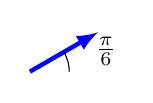
\begin{tikzpicture} \draw[->, ultra thick, blue,  arrows={-latex}]  (0,0) -- (0.866,0.5); \draw (0.5,0) arc (0:30:0.5) node[] at (15:1) {$\frac{\pi}{6}$}; \end{tikzpicture} & 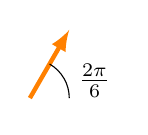
\begin{tikzpicture} \draw[->, ultra thick, orange,  arrows={-latex}]  (0,0) -- (0.5,0.866); \draw (0.5,0) arc (0:60:0.5) node[] at (15:0.85) {$\frac{2\pi}{6}$}; \end{tikzpicture} & 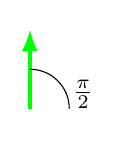
\begin{tikzpicture} \draw[->, ultra thick, green,  arrows={-latex}]  (0,0) -- (0,1); \draw (0.5,0) arc (0:90:0.5) node[] at (15:0.7){$\frac{\pi}{2}$}; \end{tikzpicture} & ... \\ 
\hline 
$\phi_k$ & 2 & 1 & 0.5 & 0.25 & ...\\ 
\hline 
$\phi_k e^{i k \theta}$ & 
\begin{tikzpicture} \draw[->, ultra thick, red,  arrows={-latex}]  (0,0) -- (2,0); \end{tikzpicture} & 
\begin{tikzpicture} \draw[->, ultra thick, blue,  arrows={-latex}]  (0,0) -- (0.866,0.5); \end{tikzpicture} & 
\begin{tikzpicture} \draw[->, ultra thick, orange,  arrows={-latex}]  (0,0) -- (0.25,0.433); \end{tikzpicture} & 
\begin{tikzpicture} \draw[->, ultra thick, green,  arrows={-latex}]  (0,0) -- (0,0.25); \end{tikzpicture} & ... \\ 
\hline 
\end{tabular} 
\end{center}
\caption{\label{tab:Summands} Example showing a step by step geometrical construction of the elements inside the summation operator in equation \ref{eq:z1complex}. In this example we use a time series whose first elements are $\phi_j = \left\lbrace 2, 1, 0.5, 0.25, ...\right\rbrace$. The parameter $\theta$ has been set to $\frac{\pi}{6}$.}
\end{table}

Adding up the elements in table \ref{tab:Summands} as indicated by equation \ref{eq:z1complex} can be interpreted geometrically as vector addition, i.e., performing one "step" after another (see figure \ref{fig:Sum}).

\begin{figure}[H]
\begin{center}
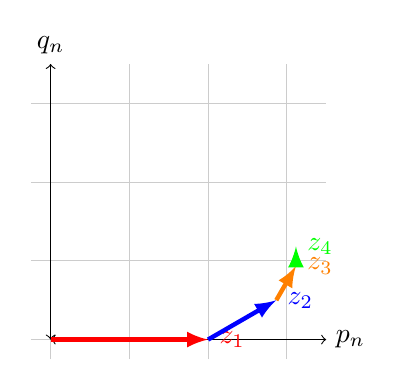
\begin{tikzpicture}
	% Grid
  	\draw[thin,gray!40] (-0.25,-0.25) grid (3.5,3.5);
  	
  	% Axes
    \draw[<->] (0,0)--(3.5, 0) node[right]{$p_n$};
  	\draw[<->] (0,0)--(0, 3.5) node[above]{$q_n$};

	% Data  	
  	\draw[->, ultra thick, red,  arrows={-latex}]  (0,0) -- (2,0) node[right]{$z_1$};
  	\draw[->, ultra thick, blue,  arrows={-latex}]  (2,0) -- (2.866,0.5) node[right]{$z_2$};
  	\draw[->, ultra thick, orange,  arrows={-latex}]  (2.866,0.5) -- (3.116,0.933) node[right]{$z_3$};
  	\draw[->, ultra thick, green,  arrows={-latex}]  (3.116,0.933) -- (3.116,1.183) node[right]{$z_4$};
  	
\end{tikzpicture}
\end{center}
\caption{\label{fig:Sum} Geometrical calculation of $z_1, z_2, z_3$ and  $z_4$ for $\phi_j = \left\lbrace 2, 1, 0.5, 0.25, ...\right\rbrace$ and $\theta = \frac{\pi}{6}$.}
\end{figure}

With this picture in mind, it is easy to understand the kind of paths that different types of time series will give rise to (see figure \ref{fig:z1Path}). Constant time series generate cyclic paths (polygons) or pseudocyclic paths (polygons that do not close after a first round). Periodic or pseudoperiodic time series generate periodic or pseudoperiodic paths (note that summand in \ref{eq:z1complex} becomes then the product of two periodic/pseudoperiodic functions). Random time series generate brownian-motion-like paths. Provided that our system is deterministic, the apparent stochasticity of our observed time series is a strong indicator of chaos.

\begin{figure}
	\begin{center}
		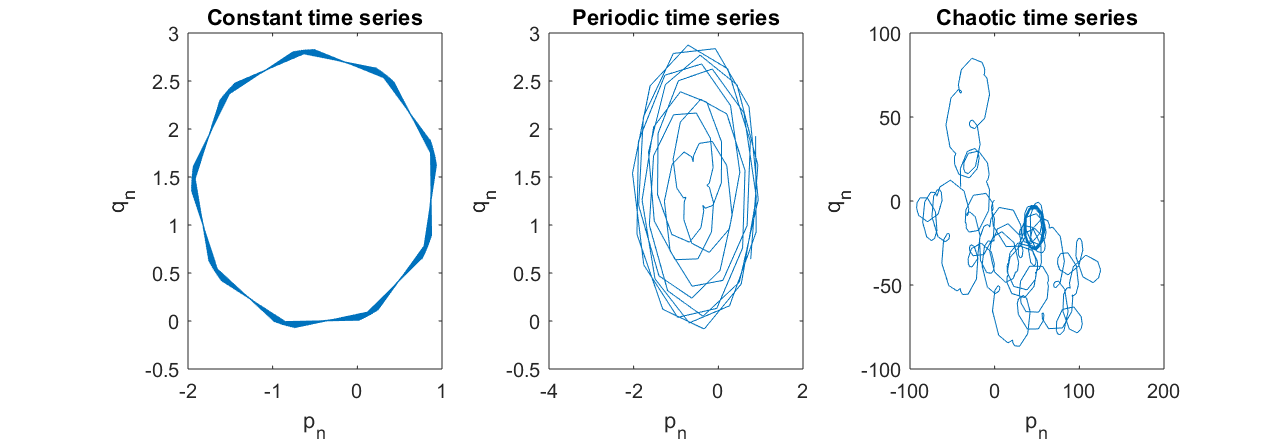
\includegraphics[width=1\columnwidth]{z1.png}
	\end{center}
	\caption{First and second panels show the paths generated by the z1 test when applied to constant and periodic time series. The third panel shows the case with a chaotic time series (notice the different scale). While in the first two cases the paths remain inside a bounded domain, in the chaotic case the path drifts away from the starting point in a brownian-motion-like fashion.}
	\label{fig:z1Path}
\end{figure}

The case of an underlying chaotic time series is the only one that generates a path that doesn't stay inside a bounded domain around the starting point. The z1 test uses the mean square displacement as a measure of this drift. The system is considered to be chaotic if the square displacement keeps growing for large times. If, on the contrary, it stays bounded, the test will consider the system not chaotic.

\subsection{Neutral competition and system dimensionality}
\label{subsec:NeutralCompetition}
If we drop everything but the competition part of our dynamics (see equation \ref{eq:SystemUnderStudy}), we will find a system of $ n_P $ equations like the following:

\begin{eqnarray}
\label{eq:OnlyCompetition}
P_i'(t) = r P_i \left( 1 - \frac{1}{K} \sum_{k=1}^{n_P} A_{ik} \cdot P_k \right) & : i = 1..n_P
\end{eqnarray}

In order to model a neutral competition, we should use the same competition coefficient for each interaction between species. That is, take $ A_{ik} = A $ for all $ i $ and $ k $. Equation \ref{eq:OnlyCompetition} then becomes:

\begin{eqnarray}
\label{eq:OnlyNeutralCompetition}
P_i'(t) = r P_i \left( 1 - \frac{A}{K} \sum_{k=1}^{n_P} P_k \right) & : i = 1..n_P
\end{eqnarray}

From equation \ref{eq:OnlyNeutralCompetition} we see that all species have exactly the same dynamical equation. This will make the nullclines to coincide at all points, so the equilibrium points will degenerate to equilibrium hyperplanes (see figure \ref{fig:Neutral}).

\begin{figure}[h]
	\begin{center}
		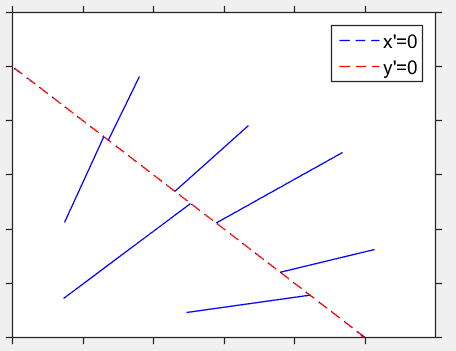
\includegraphics[width=0.9\columnwidth]{degenerate.png}
	\end{center}
	\caption{Example with $2$ prey under neutral competition. Both nullclines coincide point to point, giving rise to a higher dimensional equilibirium hyperplane (in this case, a straight line)}
	\label{fig:Neutral}
\end{figure}

This problem can be solved noticing that, in a competition-only system, the effect of neutrality is to fade out the differences between species. If this is the case, the labels $ i $ distinguishing them become meaningless. It is a natural idea to sum up all the biomasses of competing species into a new variable, that of total population of (now indistinguishable) species, defined by:

\begin{eqnarray}
\label{eq:TotalPopulation}
	T(t) = \sum_{i=1}^{n_P} P_i(t)
\end{eqnarray}

In agreement with the biological intuition, manipulating \ref{eq:TotalPopulation} and \ref{eq:OnlyNeutralCompetition} it can be proved (see eq. \ref{eq:TotalPopulationDynamics}), that the total population biomass will follow the same differential equation as the individual species abundances (i.e., equation \ref{eq:OnlyNeutralCompetition}). 

\begin{eqnarray}
\label{eq:TotalPopulationDynamics}
	 T'(t) = \sum_{i=1}^{n_P} P_i'(t) = r \sum_{i=1}^{n_P} P_i \left( 1 - \frac{A}{K} \sum_{k=1}^{n_P} P_k \right) = r T (1 - \frac{A}{K} T)
\end{eqnarray}

Additionally, this result shows that we are actually working with a one-dimensional system, because the apparent $ n_P $ dimensions of our original problem are an artifact due to a wrong choice of state variables. In our model, the predation interaction breaks this excess of symmetry, so we can still work with neutral competition as long as the predation is not neutral without facing problems of decay in system dimensionality.


\subsection{Extra figures}
\label{subsec:ExtraFigures}

\subsubsection{Flow chart}
\label{subsubsec:FlowChart}

\begin{figure}[H]
	\begin{center}
		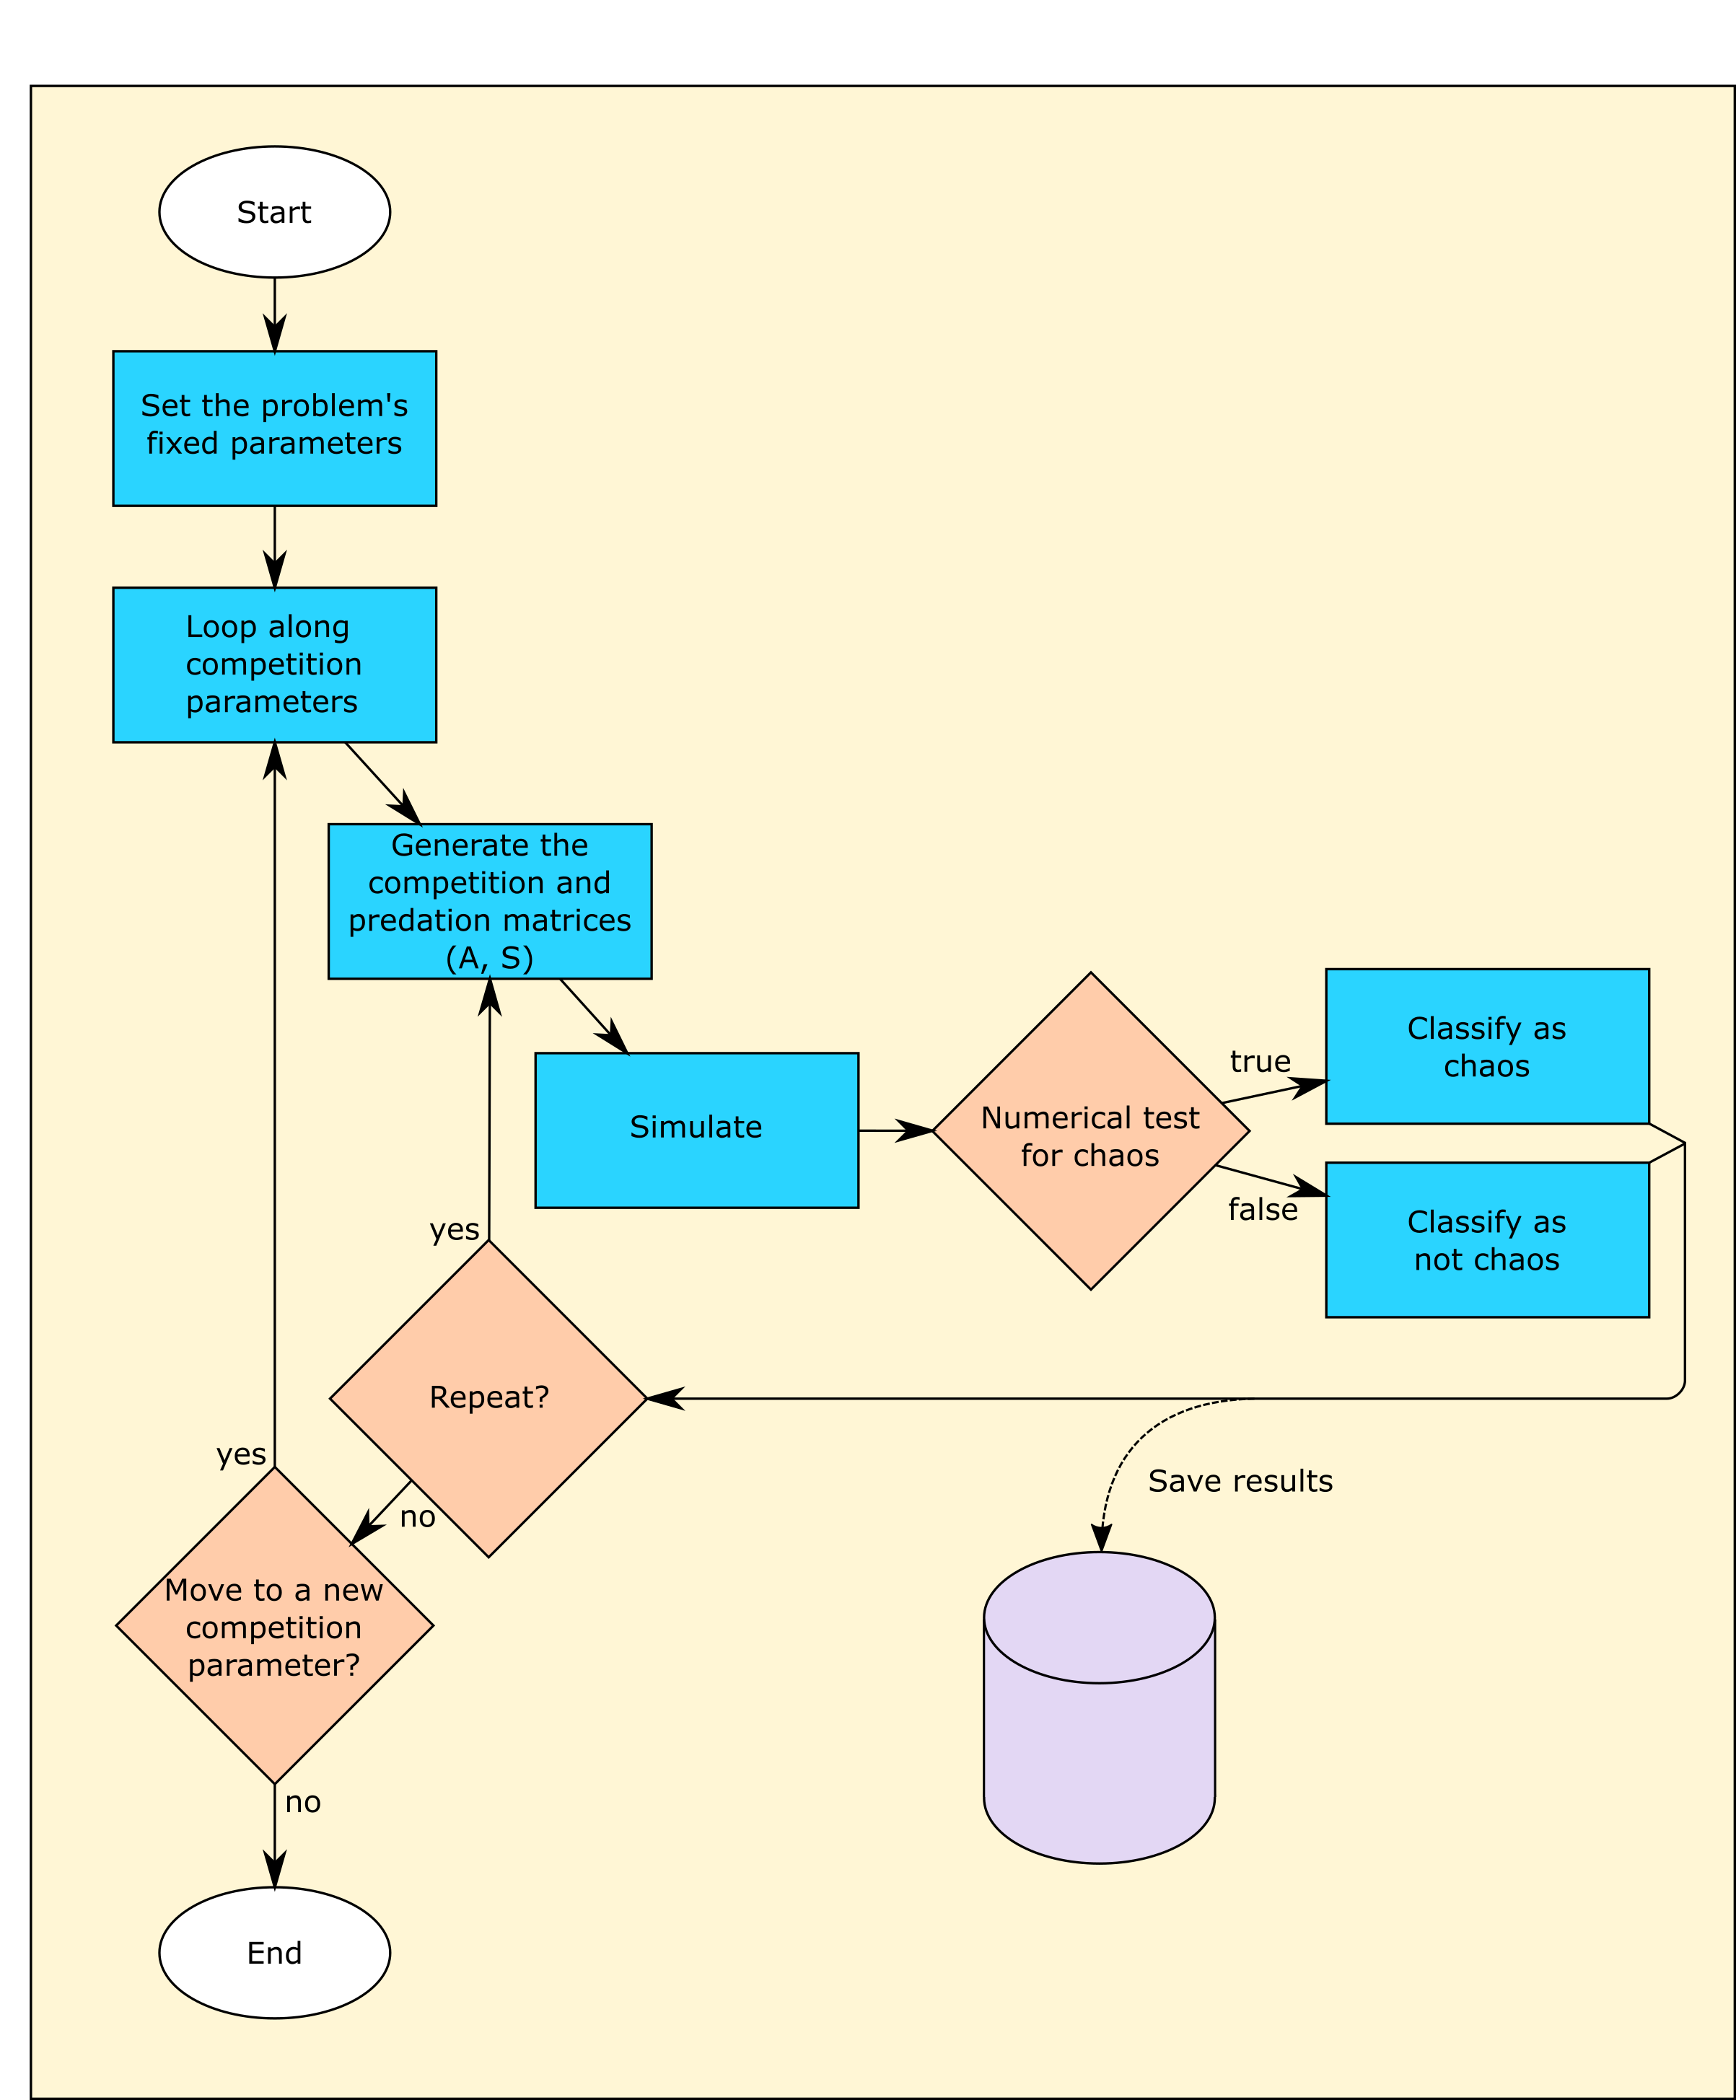
\includegraphics[width=0.9\columnwidth]{flow_chart.png}
	\end{center}
	\caption{Flow chart describing the numerical experiment. The source code is available at \textit{https://github.com/PabRod/Chaos-and-neutrality}.}
	\label{fig:FlowChart}
\end{figure}

%
%\subsection{Detection of chaos}
%\label{subsec:DetectionOfChaos}
%Dynamical systems with chaotic attractors are extremely sensitive to initial conditions. Two trajectories whose initial conditions are slightly different will diverge exponentially if they lie in the basin of a chaotic attractor. The initial rate of divergence is quantified by the Lyapunov exponent \cite{Strogatz1994}.
%
%Our procedure for classifying the attractors as chaotic or non-chaotic was based in the analysis of Lyapunov exponents. More specifically, this is the procedure we've followed:
%
%\begin{enumerate}
%	\item \label{GoToAttractor} Run the simulation for a sufficient time, in order to guarantee that a trajectory reached an attractor and the dynamics are asymptotic.
%	\item \label{RunInAttractor} Use the last point of the run in step \ref{GoToAttractor} as a starting point for a second, shorter run on the attractor.
%	\item \label{PerturbedTrajectory} Use again the last point of the run in step \ref{GoToAttractor} but, this time, adding a small disturbance to it.
%	\item Compare the runs in steps \ref{RunInAttractor} and \ref{PerturbedTrajectory} to compute numerically the principal Lyapunov exponent.
%	\begin{itemize}
%		\item If it's positive, classify the attractor as chaotic.
%		\item If it's negative, classify the attractor as non-chaotic.
%	\end{itemize}
%\end{enumerate}

\clearpage

\bibliography{../bib/library}
\bibliographystyle{vancouver}

%\listoftables
%\listoffigures

\end{document}